%%
%% prog-folien
%%
%% Slides for my Java programming tutorial using LaTeX beamer.
%%
%% Copyright (c) 2015-2016 YouniS Bensalah <younis.bensalah@gmail.com>
%%
%% This work is released to the public domain.
%% For the full copyright and license information, please view the LICENSE file.
%%

%% LaTeX-Beamer template for KIT design
%% by Erik Burger, Christian Hammer
%% title picture by Klaus Krogmann
%%
%% version 2.1
%%
%% mostly compatible to KIT corporate design v2.0
%% http://intranet.kit.edu/gestaltungsrichtlinien.php
%%
%% Problems, bugs and comments to
%% burger@kit.edu

\documentclass[18pt]{beamer}

%% SLIDE FORMAT

% use 'beamerthemekit' for standard 4:3 ratio
% for widescreen slides (16:9), use 'beamerthemekitwide'

\usepackage{templates/beamerthemekit}
% \usepackage{templates/beamerthemekitwide}

\usepackage[utf8]{inputenc}
\usepackage{hyperref}
\usepackage{listings}
\usepackage{color}
\usepackage{xcolor}
\usepackage{colortbl}
\usepackage{array}
%\usepackage{tikz}
%\usetikzlibrary{calc,shapes.multipart,chains,arrows}
\usepackage{amsmath}
\usepackage{amssymb}
\usepackage{mathrsfs}
\usepackage{eurosym}

\definecolor{lime}{HTML}{8FFF53}
\definecolor{darkgrey}{HTML}{5A5A5A}
\definecolor{awesome}{HTML}{FF2252}
\definecolor{lightgreen}{HTML}{E0FF98}

\newcommand{\quotes}[1]{``#1''}

%% TITLE PICTURE

% if a custom picture is to be used on the title page, copy it into the 'logos'
% directory, in the line below, replace 'mypicture' with the
% filename (without extension) and uncomment the following line
% (picture proportions: 63 : 20 for standard, 169 : 40 for wide
% *.eps format if you use latex+dvips+ps2pdf,
% *.jpg/*.png/*.pdf if you use pdflatex)

\titleimage{greendrop}

%% TITLE LOGO

% for a custom logo on the front page, copy your file into the 'logos'
% directory, insert the filename in the line below and uncomment it

%\titlelogo{mylogo}

% (*.eps format if you use latex+dvips+ps2pdf,
% *.jpg/*.png/*.pdf if you use pdflatex)

%% TikZ INTEGRATION

% use these packages for PCM symbols and UML classes
% \usepackage{templates/tikzkit}
% \usepackage{templates/tikzuml}

% the presentation starts here

\title[Was Ihr noch mitnehmen solltet]{Programmieren:\\ Was Ihr noch mitnehmen solltet}
\subtitle{Tutorium 30}
\author{YouniS Bensalah}
\date{February 5, 2016}

\institute{Chair for Software Design and Quality}

% Bibliography

\usepackage[citestyle=authoryear,bibstyle=numeric,hyperref,backend=biber]{biblatex}
\addbibresource{templates/example.bib}
\bibhang1em

\begin{document}

% change the following line to "ngerman" for German style date and logos
\selectlanguage{english}

%title page
\begin{frame}
\titlepage
\end{frame}

%table of contents
\begin{frame}{Heute}
\tableofcontents
\end{frame}

\section{Wiederholung}

\begin{frame}{\quad}
    \center
    \Huge{Wiederholung\\ \textbf{Java API}}
\end{frame}

\begin{frame}{Wiederholung: Java API}
    \begin{itemize}
        \item Die \textbf{Java API} ist eine Sammlung von Klassen/Paketen für häufig benötigte Funktionalitäten.

        \begin{itemize}
            \item \texttt{java.lang}: Basisfunktionalität
            \item \texttt{java.util}: Java Collections Framework
            \item \texttt{java.io}: Ein- und Ausgabe
        \end{itemize}

        \vspace{.2in}

        \item Das \textbf{Java Collections Framework} enthält u.a.
        \begin{itemize}
            \item \texttt{Map<K,V>}, \texttt{Set<E>}\dots
            \item \texttt{Queue<E>}, \texttt{Deque<E>}, \texttt{Stack<E>}\dots
            \item \texttt{List<E>}, \texttt{LinkedList<E>}\dots
        \end{itemize}

        \vspace{.2in}

        \item \quotes{Das Rad muss nicht neu erfunden werden.}

    \end{itemize}
\end{frame}

\begin{frame}{Sets und Maps}
    \begin{block}{Set}
        Ein \textbf{Set} stellt eine Menge (im mathematischen Sinne) dar: eine Sammlung von Objekten, \textit{ohne Duplikate}.
    \end{block}

    \begin{block}{Map}
        Eine \textbf{Map} stellt eine Abbildung von Schlüsseln (keys) auf Werte (values) dar.
    \end{block}
\end{frame}

\begin{frame}[fragile]{Sets}
    \begin{lstlisting}[language=Java,basicstyle=\scriptsize]
Set<String> names = new HashSet<>();

names.add("Alice");
names.add("Eve");
names.add("Bob");
names.add("Eve");

it = names.iterator();
String name;
while (it.hasNext()) {
    name = it.next();
    System.out.println(name);
}
    \end{lstlisting}

\end{frame}

\begin{frame}[fragile]{Sets}
    \begin{exampleblock}{Output}
        \begin{lstlisting}[language=Java]
Bob
Eve
Alice
        \end{lstlisting}
    \end{exampleblock}

\end{frame}


\begin{frame}[fragile]{Maps}
    \begin{lstlisting}[language=Java,basicstyle=\scriptsize]
Map<String, Integer> mountains = new HashMap<>();

mountains.put("Everest", 8848);
mountains.put("K2", 8611);
mountains.put("Kangchenjunga", 8586);
mountains.put("Lhotse", 8516);

System.out.println(mountains.get("Everest"));
    \end{lstlisting}
\end{frame}

\begin{frame}[fragile]{Maps}

    \begin{exampleblock}{Output}
        \begin{lstlisting}[language=Java]
8848
        \end{lstlisting}

    \end{exampleblock}
\end{frame}


\begin{frame}[fragile]{Stack}
    \begin{lstlisting}[language=Java,basicstyle=\scriptsize]
Stack<String> books = new Stack<>();

books.push("Modern Operating Systems");
books.push("The Magic Garden Explained");

System.out.println(books.peek());
books.pop();

books.push("The Art of Game Design");

String next;
while (!books.empty()) {
    next = books.pop();
    System.out.println(next);
}
    \end{lstlisting}

\end{frame}

\begin{frame}[fragile]{Stack}
    \begin{exampleblock}{Output}
        \begin{lstlisting}[language=Java]
The Magic Garden Explained
The Art of Game Design
Modern Operating Systems
        \end{lstlisting}
    \end{exampleblock}

\end{frame}

\begin{frame}{\quad}
    \center
    \Huge{Wiederholung\\ \textbf{Linked Lists}}
\end{frame}

\begin{frame}{Wiederholung: Linked Lists}
    \begin{block}{Verkettete Listen}
        Eine \textbf{verkettete Liste} ist eine dynamische Datenstruktur, bei der jedes Element auf seinen Nachbarn verweist.
    \end{block}

    \begin{itemize}
        \item Verkettete Listen sind ein \textit{rekursiver Datentyp}.
        \item Bei einer \textbf{einfach verketteten Liste} zeigt jedes Element auf das nächste Element in der Liste.
        \item Jedes Element enthält auch den eigentlichen Inhalt der Zelle.
        \item Das letzte Element zeigt auf \texttt{null}.
    \end{itemize}

    \begin{figure}
        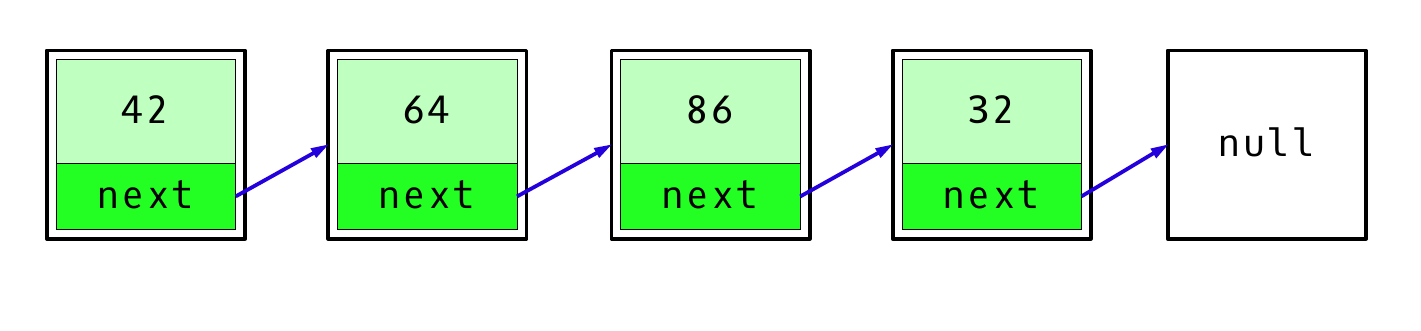
\includegraphics[scale=.3]{img/simplelinkedlist.png}
    \end{figure}
\end{frame}

\begin{frame}{Wiederholung: Linked Lists}
    \begin{itemize}
        \item Operationen auf verkettete Listen
        \begin{itemize}
            \item \textbf{Einfügen} von Listenelementen\\
            \texttt{addFirst}, \texttt{addLast}
            \item \textbf{Löschen} von Listenelementen\\
            \texttt{remove}
            \item \textbf{Suchen} nach Listenelementen\\
            \texttt{contains}
            \item \dots
        \end{itemize}
    \end{itemize}

\end{frame}

\begin{frame}{Wiederholung: Linked Lists}
    \begin{itemize}
        \item Doppelt verkettete Listen
        \begin{itemize}
            \item Jedes \textbf{Listenelement} merkt sich sowohl das \textbf{nächste} (\texttt{next}) als auch das \textbf{vorherige} (\texttt{prev}) Element
            \item \textbf{Liste} merkt sich dann sowohl \textbf{Anfang} (\texttt{head}) als auch \textbf{Ende} (\texttt{tail}) der Liste
            \item Liste kann \textit{vorwärts} wie \textit{rückwärts} traversiert werden
            \item \texttt{addLast}-Operation jetzt in $\mathcal{O}(1)$ möglich !
        \end{itemize}
    \end{itemize}

    \begin{figure}
        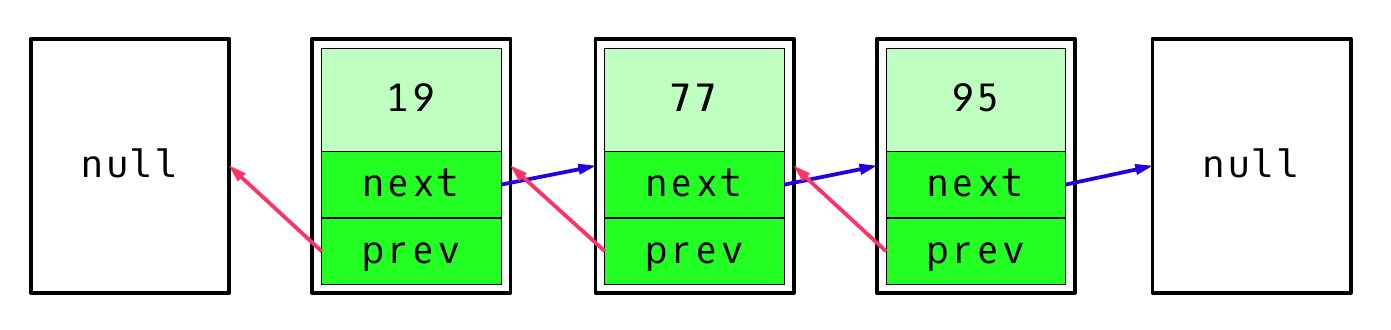
\includegraphics[scale=.3]{img/doublelinkedlist.png}
    \end{figure}

\end{frame}

\begin{frame}[fragile]{Wiederholung: Linked Lists}
    \begin{itemize}
        \item Eine (hoffentlich sinnvolle) Implementierung war die praktische Aufgabe \texttt{SuperList<Item>},
        bei welcher folgendes Interface implementiert werden sollte:
        \begin{lstlisting}[language=Java,basicstyle=\scriptsize]
public void addFirst(Item element);
public void addLast(Item element);
public void remove(Item element);
public boolean contains(Item element);
public int size();
public int count(Item element);
        \end{lstlisting}

\pause
        \item Der Code liegt immer noch auf\\ \url{http://younishd.fr/prog/superlist9k.zip}

        \item In der Java API:\quad \texttt{LinkedList<E>}

    \end{itemize}
\end{frame}

\begin{frame}{\quad}
    \center
    \Huge{Wiederholung\\ \textbf{Polymorphismus}}
\end{frame}

\begin{frame}{Wiederholung: Polymorphismus}

    \begin{itemize}
        \item Sei \texttt{Fruit} eine Klasse
        \item \texttt{Mango}, \texttt{Ananas}, \texttt{Orange} seien Unterklassen von \texttt{Fruit}
        \item Alle Objekte vom Typ \texttt{Fruit} sollen eine Methode \texttt{consume()} haben
        \item Die Methode \texttt{consume()} muss in jeder Unterklasse (\texttt{Mango}, \texttt{Ananas}, \texttt{Orange}\dots) \textit{unterschiedlich} implementiert werden
        \item Unterklassen von \texttt{Fruit} können sich also beim Aufruf von \texttt{consume()} \textit{unterschiedlich} verhalten
        \item \textbf{Problem:} \texttt{consume()} kann nicht sinnvoll in \texttt{Fruit} implementiert werden !
    \end{itemize}

    \begin{block}{}
        \begin{itemize}
            \item Eine Methode ist \textbf{polymorph}, wenn sie in verschiedenen Klassen die gleiche Signatur hat, jedoch erneut implementiert ist.
            \item Dieses Konzept bezeichnet man als \textbf{Polymorphismus}.
        \end{itemize}
    \end{block}

\end{frame}

\begin{frame}[fragile]{Wiederholung: Overriding}
    \begin{exampleblock}{}
        \begin{lstlisting}[language=Java,basicstyle=\scriptsize]
public class Orange extends Fruit {

    @Override
    public void consume() {
        System.out.println("Peel first, then eat.");
    }

}
        \end{lstlisting}

    \end{exampleblock}

\end{frame}

\begin{frame}[fragile]{Wiederholung: Overloading vs. Overriding}
    \begin{columns}[c]
        \column{.5\textwidth}
        \begin{exampleblock}{Overloading}
            \begin{lstlisting}[language=Java,basicstyle=\scriptsize]
public class Color {

    public Color(
        int red, int green, int blue)
        { ... }

    public Color(String hex) { ... }

}
            \end{lstlisting}

        \end{exampleblock}

        \column{.5\textwidth}

        \begin{exampleblock}{Overriding}
            \begin{lstlisting}[language=Java,basicstyle=\scriptsize]
public class Fruit {

    public void consume() { ... }

}

public class Ananas extends Fruit {

    @Override
    public void consume() { ... }

}
            \end{lstlisting}

        \end{exampleblock}

    \end{columns}
\end{frame}


\begin{frame}{\quad}
    \center
    \Huge{Wiederholung\\ \textbf{Misc.}}
\end{frame}

\begin{frame}[fragile]{Wiederholung: String.split()}
    \begin{lstlisting}[language=Java]
String[] split(String regex)
    \end{lstlisting}


    \begin{itemize}
        \item \texttt{String.split} zerlegt eine Zeichenkette nach einem gegebenen Muster
        \item Als Rückgabe erhält man einen Array mit den einzelnen Stücken
    \end{itemize}

\begin{exampleblock}{}
    \begin{lstlisting}[language=Java,basicstyle=\scriptsize]
String colors = "cyan;yellow;magenta";
String[] result = colors.split(";");
    \end{lstlisting}
\end{exampleblock}

\begin{itemize}
    \item Der Array \texttt{result} enthält jetzt\\ \texttt{\{ "cyan", "yellow", "magenta" \}}
\end{itemize}

\end{frame}

\begin{frame}{Wiederholung: Gleichheit von Objekten ("==" vs. equals)}
    \begin{itemize}
        \item In Java gibt es zwei Möglichkeiten, auf Gleichheit zu prüfen
        \begin{itemize}
            \item \texttt{"=="}\\
            Prüft auf Wert-Gleichheit

            \item \texttt{equals}\\
            Prüft auf inhaltliche Objekt-Gleichheit
        \end{itemize}
        \item Klasse kann \texttt{equals}-Methode \textbf{überladen} und Gleichheit von zwei Objekten selbst definieren
        \item \alert{Bei \textbf{Objekten} ist Wert-Gleichheit gerade \textbf{Gleichheit der Referenz} !}
    \end{itemize}
\end{frame}

\section{Typische Probleme und hoffentlich sinnvolle Lösungen}

\begin{frame}{\quad}
    \center
    \Huge{\textbf{Typische Probleme und hoffentlich sinnvolle Lösungen}}
\end{frame}

\begin{frame}{\quad}
    \center
    Was auch immer das heißen soll \dots
\end{frame}

\begin{frame}{Regular Expressions}
    \begin{block}{Regular Expressions}
        Reguläre Ausdrücke sind Zeichenketten, die ein Muster zum \textit{Suchen} und \textit{Ersetzen} von Text beschreiben.
    \end{block}

    \begin{itemize}
        \item Beispiele
        \begin{itemize}
            \item \textbf{Suche}: \textit{Alle Wörter, die auf \quotes{m} enden.}
            \item \textbf{Ersetze}: \textit{Alle Wörter \quotes{keyboard} durch \quotes{leopard}.}
            \item \textbf{Teste}: \textit{Enthält dieser Text ein Zeichen aus der Menge \quotes{0} \dots \quotes{9} ?}
        \end{itemize}

        \item In Java: \texttt{java.util.regex.Matcher} und \texttt{java.util.regex.Pattern} oder \texttt{String.matches()}
        \item Regex sind sehr mächtig und können oft praktisch sein
        \begin{itemize}
            \item Einfaches Parsen
            \item Eingabe auf Gültigkeit checken
            \item Text nach Wort/Muster durchsuchen
        \end{itemize}

    \end{itemize}



\end{frame}


\begin{frame}[fragile]{Crashkurs: Java Regex}
    \begin{itemize}
        \item Erstelle \texttt{Pattern} von Regex-\texttt{String}
    \begin{lstlisting}[language=Java,basicstyle=\scriptsize]
String regex = "Your regex goes here";
Pattern pattern = Pattern.compile(regex);
    \end{lstlisting}
        \vspace{.2in}
        \item Erzeuge \texttt{Matcher} ausgehend von einem \texttt{Pattern} und einem Eingabe-\texttt{String}

        \begin{lstlisting}[language=Java,basicstyle=\scriptsize]
String subject = "Your input text goes here";
Matcher matcher = pattern.matcher(subject);
        \end{lstlisting}

    \end{itemize}

\end{frame}

\begin{frame}[fragile]{Crashkurs: Java Regex}
    \begin{itemize}
        \item Ein erstes Beispiel \dots
        \begin{lstlisting}[language=Java,basicstyle=\scriptsize]
String regex = "Bar|Barbier|Rhabarber";
String subject = "Bar";
Pattern pattern = Pattern.compile(regex);
Matcher matcher = pattern.matcher(subject);
System.out.println(matcher.matches() ? "Yes" : "No");
        \end{lstlisting}
        \begin{exampleblock}{}
Yes
        \end{exampleblock}

    \end{itemize}
\end{frame}





\begin{frame}[fragile]{Crashkurs: Java Regex}
    \begin{itemize}
        \item \dots oder kürzer (mit \texttt{String.matches})

        \begin{lstlisting}[language=Java,basicstyle=\scriptsize]
String regex = "Bar|Barbier|Rhabarber";
String subject = "Bar";
System.out.println(subject.matches(regex) ? "Yes" : "No");
        \end{lstlisting}

        \begin{exampleblock}{}
Yes
        \end{exampleblock}

    \end{itemize}
\end{frame}

\begin{frame}[fragile]{Crashkurs: Java Regex}
    \begin{itemize}
        \item \Large{\quotes{\alert{\texttt{A|B}}}} : Match A or B

        \vspace{.2in}

        \begin{lstlisting}[language=Java,basicstyle=\scriptsize]
regex = "Bar|Barbier|Rhabarber";

subject = "Bar";
subject.matches(regex);  // Yes

subject = "Barbier";
subject.matches(regex);  // Yes

subject = "Rhabarber";
subject.matches(regex);  // Yes

subject = "Limonade";
subject.matches(regex);  // No
        \end{lstlisting}

    \end{itemize}
\end{frame}

\begin{frame}[fragile]{Crashkurs: Java Regex}
    \begin{itemize}
        \item \Large{\quotes{\alert{\texttt{A?}}}} : Match A 0 or 1 times

        \vspace{.2in}

        \begin{lstlisting}[language=Java,basicstyle=\scriptsize]
regex = "Bar(bara)?";

subject = "Bar";
subject.matches(regex);  // Yes

subject = "Barbara";
subject.matches(regex);  // Yes

subject = "bara";
subject.matches(regex);  // No
        \end{lstlisting}

    \end{itemize}
\end{frame}

\begin{frame}[fragile]{Crashkurs: Java Regex}
    \begin{itemize}
        \item \Large{\quotes{\alert{\texttt{A*}}}} : Match A 0 or more times

        \vspace{.2in}

        \begin{lstlisting}[language=Java,basicstyle=\scriptsize]
regex = "Bar(bara)*";

subject = "Bar";
subject.matches(regex);  // Yes

subject = "Barbara";
subject.matches(regex);  // Yes

subject = "Barbarabarabarabarabarabarabarabara";
subject.matches(regex);  // Yes

subject = "bara";
subject.matches(regex);  // No
        \end{lstlisting}

    \end{itemize}
\end{frame}

\begin{frame}[fragile]{Crashkurs: Java Regex}
    \begin{itemize}
        \item \Large{\quotes{\alert{\texttt{A+}}}} : Match A 1 or more times

        \vspace{.2in}

        \begin{lstlisting}[language=Java,basicstyle=\scriptsize]
regex = "Bar(bara)+";

subject = "Bar";
subject.matches(regex);  // No

subject = "Barbara";
subject.matches(regex);  // Yes

subject = "Barbarabarabarabarabarabarabarabara";
subject.matches(regex);  // Yes

subject = "bara";
subject.matches(regex);  // No
        \end{lstlisting}

    \end{itemize}
\end{frame}

\begin{frame}[fragile]{Crashkurs: Java Regex}
    \begin{itemize}
        \item \Large{\quotes{\alert{\texttt{A\{n\}}}}} : Match A exactly n times

        \vspace{.2in}

        \begin{lstlisting}[language=Java,basicstyle=\scriptsize]
regex = "Bar(bara){3}";

subject = "Bar";
subject.matches(regex);  // No

subject = "Barbara";
subject.matches(regex);  // No

subject = "Barbarabarabara";
subject.matches(regex);  // Yes

subject = "Barbarabarabarabarabarabarabarabara";
subject.matches(regex);  // No
        \end{lstlisting}

    \end{itemize}
\end{frame}

\begin{frame}[fragile]{Crashkurs: Java Regex}
    \begin{itemize}
        \item \Large{\quotes{\alert{\texttt{A\{n,\}}}}} : Match A at least n times

        \vspace{.2in}

        \begin{lstlisting}[language=Java,basicstyle=\scriptsize]
regex = "Bar(bara){3,}";

subject = "Bar";
subject.matches(regex);  // No

subject = "Barbara";
subject.matches(regex);  // No

subject = "Barbarabarabara";
subject.matches(regex);  // Yes

subject = "Barbarabarabarabarabarabarabarabara";
subject.matches(regex);  // Yes
        \end{lstlisting}

    \end{itemize}
\end{frame}

\begin{frame}[fragile]{Crashkurs: Java Regex}
    \begin{itemize}
        \item \Large{\quotes{\alert{\texttt{A\{n,m\}}}}} : Match A at least n but no more than m times

        \vspace{.2in}

        \begin{lstlisting}[language=Java,basicstyle=\scriptsize]
regex = "Bar(bara){3,5}";

subject = "Barbarabara";
subject.matches(regex);  // No

subject = "Barbarabarabara";
subject.matches(regex);  // Yes

subject = "Barbarabarabarabara";
subject.matches(regex);  // Yes

subject = "Barbarabarabarabarabara";
subject.matches(regex);  // Yes

subject = "Barbarabarabarabarabarabara";
subject.matches(regex);  // No
        \end{lstlisting}

    \end{itemize}
\end{frame}


\begin{frame}[fragile]{Crashkurs: Java Regex}
    \begin{itemize}
        \item \Large{\quotes{\alert{\texttt{$\left[abc\right]$}}}} : Match a character class

        \vspace{.2in}

        \begin{lstlisting}[language=Java,basicstyle=\scriptsize]
regex = "B[abc]rbara";

subject = "Barbara";
subject.matches(regex);  // Yes

subject = "Bbrbara";
subject.matches(regex);  // Yes

subject = "Bcrbara";
subject.matches(regex);  // Yes

subject = "Bxrbara";
subject.matches(regex);  // No
        \end{lstlisting}

    \end{itemize}
\end{frame}

\begin{frame}[fragile]{Crashkurs: Java Regex}
    \begin{itemize}
        \item \Large{\quotes{\alert{\texttt{$\left[a-z\right]$}}}} : Match a character class (range)

        \vspace{.2in}

        \begin{lstlisting}[language=Java,basicstyle=\scriptsize]
regex = "B[a-z]rbara";

subject = "Barbara";
subject.matches(regex);  // Yes

subject = "Bbrbara";
subject.matches(regex);  // Yes

subject = "Byrbara";
subject.matches(regex);  // Yes

subject = "Bzrbara";
subject.matches(regex);  // Yes
        \end{lstlisting}

    \end{itemize}
\end{frame}

\begin{frame}[fragile]{Crashkurs: Java Regex}
    \begin{itemize}
        \item \Large{\quotes{\alert{\texttt{$\left[\wedge abc\right]$}}}} : Match a character class (negation)

        \vspace{.2in}

        \begin{lstlisting}[language=Java,basicstyle=\scriptsize]
regex = "B[^def]rbara";

subject = "Barbara";
subject.matches(regex);  // Yes

subject = "Bdrbara";
subject.matches(regex);  // No

subject = "Berbara";
subject.matches(regex);  // No

subject = "Bfrbara";
subject.matches(regex);  // No

subject = "Bgrbara";
subject.matches(regex);  // Yes
        \end{lstlisting}

    \end{itemize}
\end{frame}

\begin{frame}[fragile]{Crashkurs: Java Regex}
    \begin{itemize}
        \item \Large{\quotes{\alert{\texttt{$.$}}}} : Match any character

        \vspace{.2in}

        \begin{lstlisting}[language=Java,basicstyle=\scriptsize]
regex = "B.rbara";

subject = "Barbara";
subject.matches(regex);  // Yes

subject = "Bxrbara";
subject.matches(regex);  // Yes

subject = "Byrbara";
subject.matches(regex);  // Yes

subject = "B4rbara";
subject.matches(regex);  // Yes

subject = "Baaaarbara";
subject.matches(regex);  // No
        \end{lstlisting}

    \end{itemize}
\end{frame}

\begin{frame}[fragile]{Crashkurs: Java Regex}
    \begin{itemize}
        \item \Large{\quotes{\alert{\texttt{$(A)$}}}} : Extract a matched group

        \vspace{.2in}

        \begin{lstlisting}[language=Java,basicstyle=\scriptsize]
regex = "Bar(.*)bara";
Pattern pattern = Pattern.compile(regex);
Matcher match;

matcher = pattern.matcher("Barxyzbara");
if (matcher.find()) {
    System.out.print( subject.group(1) );  // "xyz"
}

matcher = pattern.matcher("Barbara");
if (matcher.find()) {
    System.out.print( subject.group(1) );  // "" (empty string)
}

matcher = pattern.matcher("Limonade");
if (matcher.find()) {  // no match: find() returns false
    System.out.print( subject.group(1) );
}
        \end{lstlisting}

    \end{itemize}
\end{frame}


\begin{frame}{Regular Expressions}
    \begin{itemize}
        \item Mehr zu Java Regex hier:
        \vspace{.2in}
        \begin{itemize}
            \item \url{https://docs.oracle.com/javase/tutorial/essential/regex}
            \item \url{https://docs.oracle.com/javase/8/docs/api/java/util/regex/Pattern.html}
            \item \url{https://docs.oracle.com/javase/8/docs/api/java/util/regex/Matcher.html}
            \item \url{http://www.ocpsoft.org/opensource/guide-to-regular-expressions-in-java-part-1}
        \end{itemize}
    \end{itemize}
\end{frame}


\begin{frame}[fragile]{Regular Expressions}
    \begin{itemize}
        \item Codeschnipsel aus meiner eigenen Prog. Abschlussaufgabe\dots
    \end{itemize}
    \begin{lstlisting}[language=Java,basicstyle=\tiny]
String regex =
    "^\\s*(?<subjectName>[a-zA-Z0-9]+)(?>\\s*\\(\\s*id\\s*=\\s*(?<subjectId>[0-9]+)\\s*\\))?\\s+"
    + "(?<predicate>contains|contained-in|part-of|has-part|successor-of|predecessor-of)\\s+"
    + "(?<objectName>[a-zA-Z0-9]+)(?>\\s*\\(\\s*id\\s*=\\s*(?<objectId>[0-9]+)\\s*\\))?\\s*$";

this.pattern = Pattern.compile(regex);

// ...

Matcher matcher = this.pattern.matcher(line);
    \end{lstlisting}

\begin{itemize}
    \item Die Regex hat dann solche Textdateien geparst\dots
\end{itemize}

    \begin{lstlisting}[language=Java,basicstyle=\tiny]
CentOS7 (id=107) contained-in OperatingSystem
officesuite contained-in Software
LibreOffice (id=200) contained-in officesuite
writer (id=201) part-of LibreOffice (id=200)
libreoffice (id=200) has-part impress (id=203)
...
    \end{lstlisting}




    \begin{figure}
        
\includegraphics[scale=.1]{img/dealwithit.jpg}
    \end{figure}

\end{frame}


\begin{frame}{Regular Expressions}
    \begin{figure}
        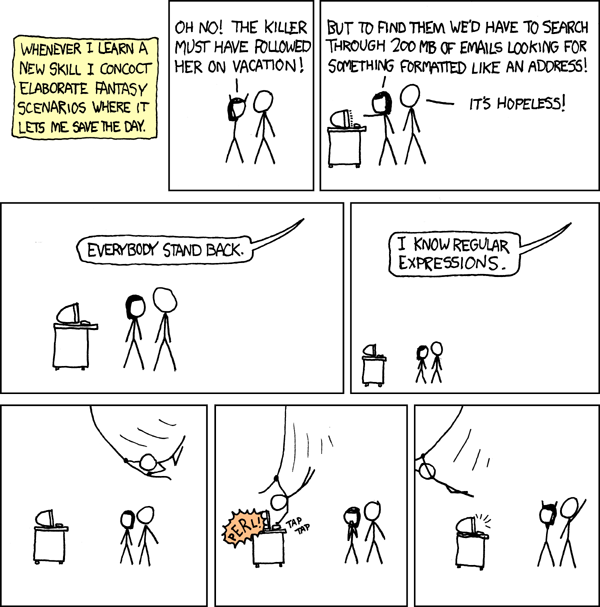
\includegraphics[scale=.3]{img/regular_expressions.png}
    \end{figure}
\end{frame}



\begin{frame}[fragile]{Duplikate in Array/List}
    \begin{itemize}
        \item \textbf{Problem:} Bestimme, ob ein \texttt{Array} bzw. eine \texttt{List} doppelte Elemente enthält.
        \vspace{.2in}
    \begin{lstlisting}[language=Java,basicstyle=\scriptsize]
String[] fruitArray = {
    "Apfel",
    "Mango",
    "Ananas",
    "Orange",
    "Apfel",
    "Kiwi",
    "Birne",
    "Apfel",
    "Orange"
};
    \end{lstlisting}

    \end{itemize}

\end{frame}

\begin{frame}[fragile]{Duplikate in Array/List}
    \begin{itemize}
        \item \textbf{Lösung:} Füge alle Elemente in ein \texttt{Set} ein und vergleiche dann die Größe von \texttt{Set} und \texttt{Array}.

\vspace{.2in}

        \begin{lstlisting}[language=Java,basicstyle=\scriptsize]
String[] fruitArray = { ... };

Set<String> fruitSet = new HashSet<>(Arrays.asList(fruitArray));

if (fruitSet.size() == fruitArray.length) {
    System.out.println("No duplicates.");
} else {
    System.out.println("Duplicates.");
}
        \end{lstlisting}

\begin{exampleblock}{}
\begin{lstlisting}[language=Java,basicstyle=\scriptsize]
Duplicates.
\end{lstlisting}

\end{exampleblock}


    \end{itemize}
\end{frame}


\begin{frame}[fragile]{Klammern}
    \begin{itemize}
        \item \textbf{Problem:} Bestimme, ob ein Klammerausdruck gültig ist.
    \end{itemize}
\end{frame}

\begin{frame}[fragile]{Klammern}
    \begin{itemize}
        \item \textbf{Lösung:} Verwende einen \texttt{Stack} !
    \end{itemize}

    \begin{lstlisting}[language=Java,basicstyle=\scriptsize]
boolean parseParens(String input) {
    Stack<Character> parens = new Stack<>();
    for (int i = 0; i < input.length(); i++) {
        char c = input.charAt(i);
        if (c == '(') {
            parens.push('(');
        } else if (c == ')') {
            if (parens.empty() || parens.peek() != '(') {
                return false;
            }
            parens.pop();
        } else {
            return false;
        }
    }
    return parens.empty();
}

parseParens("(())()((()()))()");  // true
parseParens("(()()))()(");  // false
    \end{lstlisting}

\end{frame}



\appendix
\beginbackup

\begin{frame}{Fragen ?}
    \begin{figure}
        
\includegraphics[scale=.4]{img/iknowjava.jpg}
    \end{figure}
\end{frame}

\begin{frame}{Viel Erfolg bei den Abschlussaufgaben !}
    \center
    \textsc{\quotes{Think first, code later.}}
    \begin{figure}
        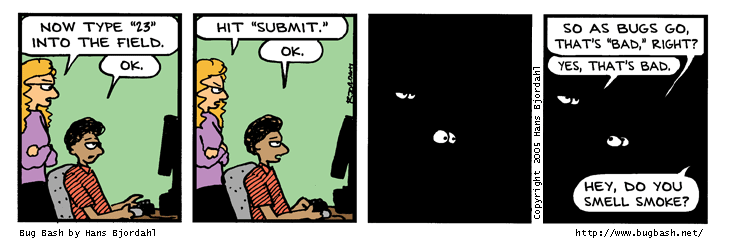
\includegraphics[scale=.6]{img/bug-bash20050521.png}
    \end{figure}
\end{frame}

\backupend

\end{document}
